\documentclass[10pt]{scrreprt}

\usepackage{cmap}

\usepackage[utf8]{inputenc}
\usepackage[T1]{fontenc}
\usepackage[english, ngerman]{babel}

\usepackage{afterpage}
\usepackage{amsmath}
\usepackage{amsthm}
\usepackage{amsfonts}
\usepackage{csquotes}
\usepackage{enumerate}
\usepackage{geometry}
\usepackage{mathtools}
\usepackage{mdframed}
\usepackage{microtype}
\usepackage{sgame}
\usepackage{tikz} 
\usepackage{titlesec}
\usepackage{xpatch}
\usetikzlibrary{hobby}

%standard setup
\author{Martin Belica ~\\ {\large im Auftrag von fuks e.V.} ~}
\date{Wintersemester 2018}
\publishers{Karlsruher Institut für Technologie}
\title{{\Large Crashkurs} \\ Volkswirtschaftslehre I - Mirkoökonomie}

\pdfinfo{
        /Author (Martin Belica)
        /Title   (Crashkurs Volkswirtschaftslehre I - Mirkoökonomie)
        /Subject (Volkswirtschaftskehre I)
        /Keywords (Crashkurs, Volkswirtschaftslehre, Mirkoökonomie, VWLI)
}

\makeatletter
	\setlength{\parindent}{0cm}
	\xpatchcmd{\proof}{\@addpunct{.}}{\@addpunct{:}}{}{}
	\titleclass{\chapter}{straight}
	\titleformat{\chapter}{\bfseries\huge}{\thechapter}{0.4em}{}
	\titlespacing*{\chapter}{0mm}{3em}{1em}
\makeatother

\newcounter{thm}
\newtheoremstyle{thmstyle}
  {0.25em} % Space above
  {1.25em} % Space below
  {} % Body font
  {} % Indent amount
  {\bfseries} % Theorem head font
  {: } % Punctuation after theorem head
  {0em} % Space after theorem head
  {} % Theorem head spec (can be left empty, meaning `normal')
\theoremstyle{thmstyle} 
\numberwithin{thm}{chapter}

\newtheorem*{beispiel}{Beispiel}
\newtheorem*{krb}{KR}

\newenvironment{kr}
  {\begin{mdframed}\begin{krb}}
  {\end{krb}\end{mdframed}}
  
  
\begin{document}

\pagenumbering{arabic}
\setcounter{page}{1}

\maketitle

\afterpage{%
\newgeometry{top=3.5cm,bottom=3.5cm,outer=2.5cm,inner=2.5cm}

\thispagestyle{empty} 
\tableofcontents ~\bigskip ~\bigskip

Dieses Skript dient der Zusammenfassung und anschaulichen Darstellung des Vorlesungsstoffes der Vorlesung VWL I - Mikroökonomie für da Wintersemester 2018/19. Der Crashkurs hat das Ziel die Studierenden bei der Prüfungsvorbereitung zu unterstützen, indem die Inhalte der Vorlesung in kompakter Form wiederholt, sowie durch Übungsaufgaben vertieft werden. Die Darstellung in kompakter Form ist als solche zu verstehen und kann daher explizit \textbf{keine Vollständigkeit} gewähren. Auch wurde versucht einen Kompromiss zwischen Exaktheit und Anschaulichkeit zu finden, der den Studierenden in der Vorbereitung helfen soll. ~\bigskip

Viele Graphiken und vertiefende Beispiele werden im Kurs gemeinsam erarbeitet, wodurch das Skript weiter vervollständigt wird. Das Durcharbeiten der Vorlesungsfolien kann allerdings durch das Studieren des vorliegenden Skriptes nicht ersetzt werden. Ebenso besteht \textbf{keine Gewähr auf die Richtigkeit} der Inhalte. Die Inhalte sind insbesondere \textbf{nicht vom Lehrstuhl geprüft}. Für eine ausführliche Ausarbeitung sei auf die Vorlesung sowie auf die in der Vorlesung empfohlene Literatur verwiesen.

\clearpage
\restoregeometry
} 

\chapter{Spieltheorie}

Die Spieltheorie analysiert Situationen mit strategischer Interaktion, in denen sich also der Nutzen, den die Akteure aus der Situation ziehen, durch individuelle Entscheidungen wechselseitig beeinflusst. ~\bigskip

Eine Allokation heißt \textbf{Pareto-Effizienz}, falls keine Akteur besser gestellt werden kann, ohne einen anderen schlechter zu stellen. Damit darf es keine andere Allokation geben, in der jeder Akteur mindestens gleich gut gestellt  und mindestens eine Person echt besser gestellt ist. Pareto-Effizienz hat allerdings nichts mit Gerechtigkeit zu tun; lediglich Verschwendung in der Verteilung darf nicht vorliegen. ~\bigskip

Ein \textbf{Spiel} ist eine strategische Interaktionssituation die durch folgenden Aspekte charakterisiert wird:
\begin{itemize}
	\item Spieler
	\item Strategien und Spielregeln für jeden Spieler
	\item Spielergebnisse bzw. Spielausgänge
	\item Nutzen aus jedem möglichen Spielergebnis
\end{itemize}

\section{Spiele in Normalform}

Die Normalform beschreibt lediglich die Spieler, Strategien und Auszahlungen eines Spiels - was für viele Spiele alle relevanten Informationen enthält. Ein solches Spiel kann durch eine Matrix dargestellt werden. ~\bigskip

Als Beispiel sei hier die Situation zweier Gefangener dargestellt, die beschuldigt werden, gemeinsam ein Verbrechen begangen zu haben. Die beiden Gefangenen werden einzeln verhört und können nicht miteinander kommunizieren.
\begin{table}[!htbp]
	\centering
	\begin{game}{2}{2}[Spieler 1][Spieler 2]
	 	   	  	   &  gestehen &  schweigen  \\
		gestehen   &  $2, 2$   & $0, 3$      \\
		schweigen  &  $3, 0$   & $1, 1$      \\
	\end{game}
\end{table}

Eine Strategie die für einen Spieler immer vorteilhaft ist - unabhängig von den Entscheidungen aller anderen Spieler - nennt man \textbf{dominante Strategie}. Spielt jeder Spieler eine dominante Strategie, so liegt ein \textbf{Gleichgewicht in dominanten} Strategien vor. ~\smallskip

Zum Ermitteln von dominanten Strategien ist es möglich die sogenannten besten Reaktionen zu verwenden. Eine Strategie ist eine \textbf{Beste Reaktion}, wenn sie den Nutzen eines Spielers - gegeben die Strategien aller anderen Spieler - maximiert.

\begin{kr}[Beste Antwort]~\
	\begin{itemize} 		
		\item In jeder Spalte wird die höchste Auszahlung von Spieler 1 unterstrichen. 
		\item In jeder Zeile wird die höchste Auszahlung von Spieler 2 unterstrichen.
	\end{itemize}	
\end{kr}

\begin{kr}[Dominante Strategie] ~\
	\begin{itemize}
		\item Eine Strategie ist für Spieler 1 dominant, falls nach KR (Beste Antwort) alle Auszahlungen in der zugehörigen Zeile unterstrichen sind.
		\item Eine Strategie ist für Spieler 2 dominant, falls nach KR (Beste Antwort) alle Auszahlungen in der zugehörigen Spalte unterstrichen sind.
	\end{itemize}	
\end{kr}

Ein \textbf{Gefangenendilemma} kennzeichnet eine Situation, in der individuell rationales Verhalten der einzelnen Spieler zu einem für die Gruppe nicht Pareto-optimialem Ergebnis führt. Es existiert dann ein Strategienpaar, das zu einer Pareto-Verbessrung führt und das nur durch Änderung der Strategien aller Spieler erreicht werden kann. ~\bigskip

Ein \textbf{Nash-Gleichgewicht in reinen Strategien} ist ein Strategienpaar, bei dem jeder Spieler die optimale Wahl trifft, gegeben der Wahl des anderen Spielers. Sie ist also die gegenseitig beste Antwort und damit will kein Spieler einseitig vom  Nash-Gleichgewicht abweichen.

\begin{kr}[Nash-Gleichgewicht in reinen Strategien] ~\\
	Das Strategienpaar das zu einer Zelle führt, in der nach KR (Beste Antwort) die Auszahlungen beider Spieler unterstrichen sind, stellt ein Nash-Gleichgewicht in reinen Strategien dar.
\end{kr}

Es muss kein Nash-Gleichgewicht in reinen Strategien geben. Ein \textbf{Nash-Gleichgewicht in gemischten Strategien} ist eine Wahrscheinlichkeitsverteilung über die reine Strategien aller Spieler von der kein Spieler einseitig abweichen möchte. 

\begin{kr}[Nash-Gleichgewicht in gemischten Strategien] ~\\
	Haben beide Spieler zwei Strategien, so kann man das Nash-Gleichgewicht in gemischten Strategien ermitteln indem man für jeden Spieler den erwarteten Nutzen seiner beiden Strategien gegeben der Wahrscheinlichkeitsverteilung gleich setzt.
\end{kr}

\section{Sequentielle Spiele}

Eine \textbf{Strategie} in sequentiellen Spielen ist ein vollständiger Aktionsplan, der zu jedem beliebigen Spielzeitpunkt die Aktion eines Spielers beschreibt.

Sequentielle Spiele werden im Allgemeinen durch Rückwärtsinduktion gelöst. Dabei werden alle Nash-Gleichgewichte identifiziert die nicht auf unglaubwürdigen Drohungen beruhen. Die resultierende Strategie definiert ein \textbf{teilspielperfektes Nash-Gleichgewicht}.

\begin{kr}[Teilspielperfekte Nash-Gleichgewichte] ~\\
	Ersetze iterativ alle letzten Entscheidungsknoten durch die glaubwürdigen Drohungen im Punkt, bis alle Knoten ersetzt sind. Alle getroffenen Entscheidungen bilden das teilspielperfekte Nash-Gleichgewicht.
\end{kr}

\section{Auktionen}

Es gibt vier Standardformen der Auktion. Sie unterscheiden sich in der Art der Gebotsabgaben, der Zuschlags- und Preisregeln:
\begin{itemize}
	\item \textbf{Englische Auktion}: Aufsteigende, offene Gebote. Höchstgebot bzw. letzter verbleibender Bieter erhält den Zuschlag. Gewinner zahl sein Gebot.
	\item \textbf{Holländische Auktion}: Absteigende Auktion. Preisvorschläge durch Auktionator fallen. Den Zuschlag erhält das erste Gebot und gezahlt wird auch das Gebot.
	\item \textbf{Erstpreisauktion}: Verdeckte, einmalige Gebotsabgabe. Höchstgebot erhält den Zuschlag. Gewinner zahlt sein Gebot.
	\item \textbf{Zweitpreisauktion} (auch Vickrey-Auktion genannt): Verdeckte, einmalige Gebotsabgabe. Hächstebot erhält den Zuschlag. Gewinner zahl das zweithächste Gebot.
\end{itemize}

\subsubsection*{Private Value Auktion}

Für diese vier Formen der Auktionen gilt das sogenannte Revenue Equivalance Theorem (RET). Sind die Bieter nämlich risikoneutral mit privaten Wertschätzungen, so erbringen alle obigen Formen in Erwartung denselben Erlös - das heißt es entsteht der selbe Verkaufspreis (\textbf{Erlösäquivalenz}). ~\bigskip

Allerdings kann es aus empirischer Sicht Sinn machen, die Erstpreis- der Zweitpreisauktion vorzuziehen. Unter Risikoaversion oder begrenzter Rationalität neigt diese zu einem höheren Erlös. ~\bigskip

Außerdem sind Zweitpreis- und Englische Auktion strategisch äquivalent. In beiden Auktionsformen gibt es die dominante Strategie seine Wertschätzung zu bieten, die weder in der Erstpreis- noch in der Holländischen Auktion dominant ist.

\subsubsection*{Common Value Auktion}
 
 Ist der Wert des Gutes für alle Bieter gleich, kennen diesen jedoch die Bieter nicht, spricht man von einer Common-Value-Auktion. ~\bigskip
 
 Jeder Bieter schätz den Wert des Gutes und basiert darauf seine Gebote. Die Durchschnittsschätzung aller Bieter ist generell ein guter Schätzer für den Wert des Gutes. Da der Zuschlag allerdings an den Höchstbietenden geht, fällt die erwartete Auszahlung des Auktionsgewinners typischerweise niedriger aus als die realisierte Auszahlung, da die Durchschnittsschätzung (\enquote{Common Value}) vom Gewinner überschätzt wird (im Extremfall können Verluste entstehen, was als \enquote{Winners' Curse} bezeichnet wird).
\chapter{Grundlagen des Angebots- und Nachfragemodells}

Ein \textbf{Markt} ist ein Mechanismus, durch den Käufer und Verkäufer interagieren um Preise festzulegen und Güter zu handeln. Wir interessieren uns allgemein für die Preisbildung am Markt sowie die Vorgänge, die zur Bildung eines Marktgleichgewichts führen. ~\bigskip

Ein \textbf{Marktgleichgewicht} liegt dann vor, wenn das Angebot der Nachfrage gleicht. Damit ist der Gleichgewichtspreis der Preis $p^*$ für den gilt:
	$$ S(p^*) = D(p^*) $$
Es ist irrelevant, ob hier Gleichheit der Angebots- und Nachfragefunkion oder deren Inversen steht.

\begin{figure*}[!htbp] \centering
	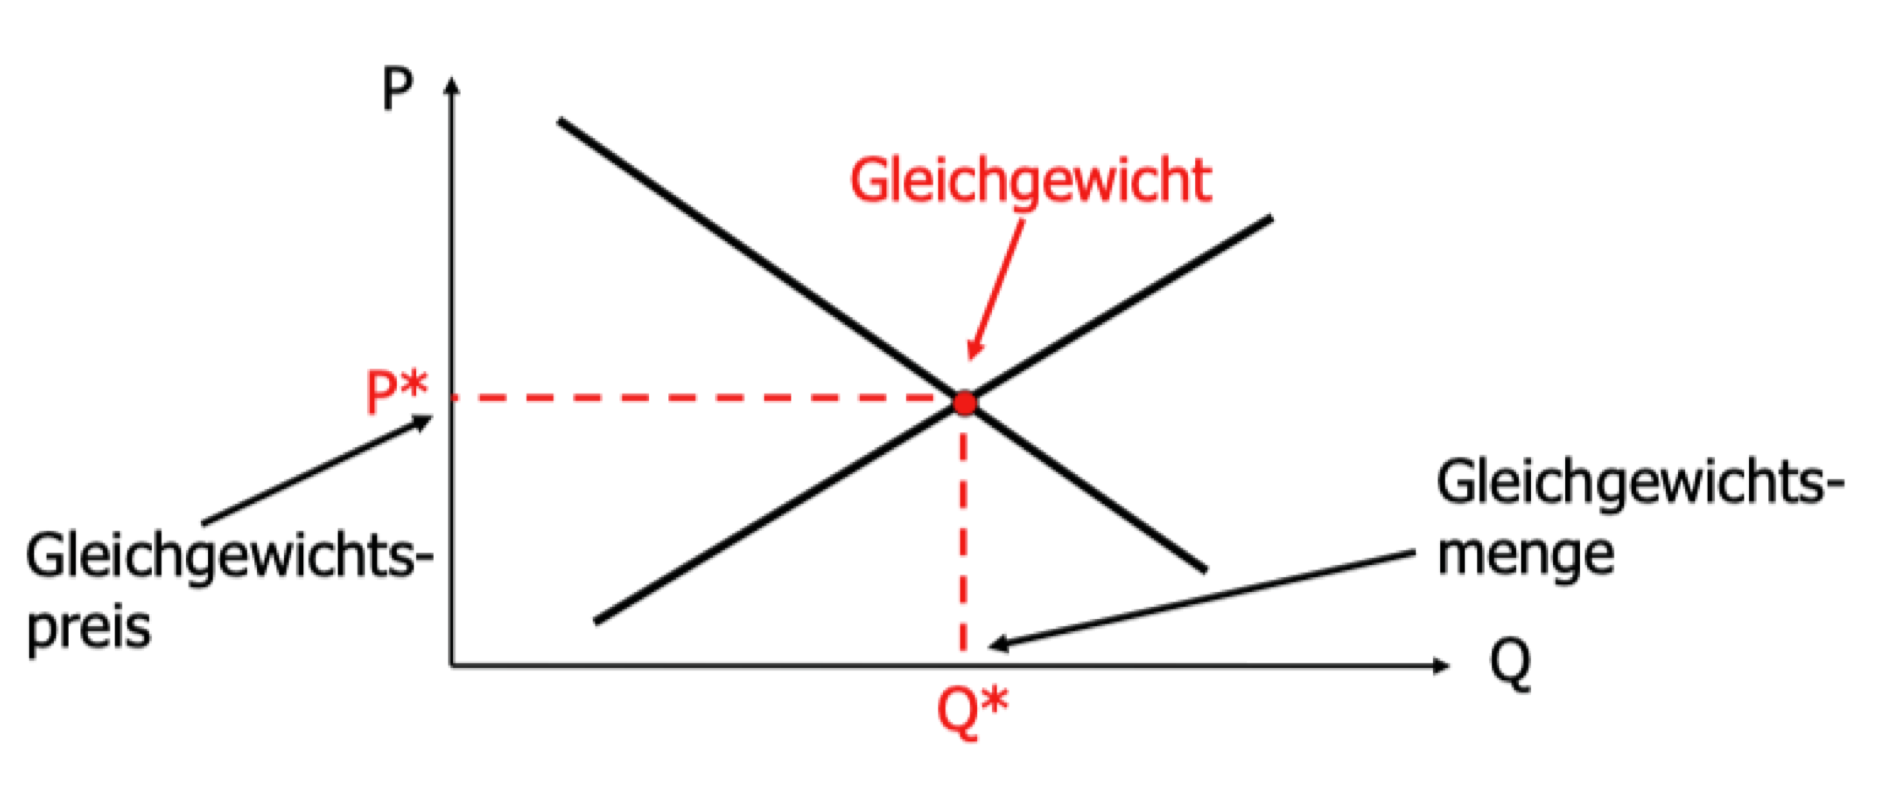
\includegraphics[scale=0.25]{img/marktgleichgewicht}
\end{figure*}

\subsubsection*{Aggregation}

Sind mehrere Anbieter oder Nachfrager auf dem Markt vertreten, so ist die Gesamtmarktnachfrage die horizontale Summe der individuellen (\textbf{Aggregation}).

\begin{kr}[Aggregation der Nachfrage] ~\\
	Bei der Aggregation mehreren Nachfragen $D_i$, die abschnittsweise durch Preise $p_i$ definiert sind, zerteile die einzelnen Nachfragen zuerst nach jedem Abschnittspreis $p_i$. Auf jedem einzelnen Abschnitt ist die aggregierte Nachfrage einfach die Summe der Einzelnachfragen.  
\end{kr}

\begin{kr}[Marktgleichgewicht bei aggregierten Nachfragen] ~\\
	Ist die Nachfrage abschnittsweise auf Preisintervallen $[\underline{p}, \overline{p})$ definiert, berechne auf jeden Abschnitt einzeln den möglichen Gleichgewichtspreis $p^*$. Ist $p^* \in [\underline{p}, \overline{p})$ so ist $p^*$ der tatsächliche Gleichgewichtspreis des aggregierten Zustands, ist allerdings $p^* \notin [\underline{p}, \overline{p})$ fahre mit dem nächsten Abschnitt fort.
\end{kr}~\newpage

\subsubsection*{Elastizitäten}

Wie empfindlich die Nachfrage auf eine Änderung eines Parameters (wie z.B. die Preise oder das Einkommens) reagiert, wird durch die entsprechende \textbf{Elastizität} ausgedrückt:
\begin{itemize}
	\item \textbf{Preiselastizität} $\hat{=}$ prozentuale Änderung der Nachfrage nach Gut $i$ im Verhältnis zur prozentualen Änderung des entsprechenden Preises: 
	$$ \epsilon_{i, p} = \epsilon_D(p_i) = \frac{\partial D}{\partial p_i} \frac{p_i}{D} $$
	Ist $|\epsilon_D| > 1$ so spricht man von einer elastischen Nachfrage, ist $|\epsilon_D| = 1$ von einer einheitselastischen und ist $|\epsilon_d| < 1$ von einer unelastischen Nachfrage.
	\item \textbf{Einkommenselastizität} $\hat{=}$ prozentuale Änderung der Nachfrage im Verhältnis zur prozentualen Änderung des Einkommens: $$ \epsilon_{i, m} = \epsilon_D(m) = \frac{\partial D}{\partial m} \frac{m}{D} $$
	\item \textbf{Kreuzpreiselastizität} $\hat{=}$ prozentuale Änderung der Nachfrage  nach Gut $i$, im Verhältnis zur prozentualen Änderung des Preises eines anderen Guts $j$: 
	$$ \epsilon_{ij} = \epsilon_{D_i}(p_j) = \frac{\partial D_i}{\partial p_j} \frac{p_j}{D_i} $$
	Wenn $\epsilon_{ij} > 0$, dann sind Gut $i$ und $j$ Substitute, und wenn $\epsilon_{ij} < 0$, dann sind Gut $i$ und $J$ Komplemente.
\end{itemize} ~\smallskip

\subsubsection*{Renten}

\begin{figure}[htbp!]
	\begin{minipage}[t]{9cm}\vspace{0pt} ~\\
		Die Differenz zwischen dem, was ein Konsument zu bezahlen bereit wäre (Zahlungsbereitschaft) und dem, was er tatsächlich zahlen muss, ist die \textbf{Konsumentenrente}. Grafisch ist die Konsumentenrente die Fläche unter der inversen Nachfragefunktion zwischen 0 und der nachgefragten Menge $x^*$ abzüglich der Ausgaben.
	\end{minipage}
	\hspace{0.25cm}
	\begin{minipage}[t]{3cm}\vspace{1pt}
		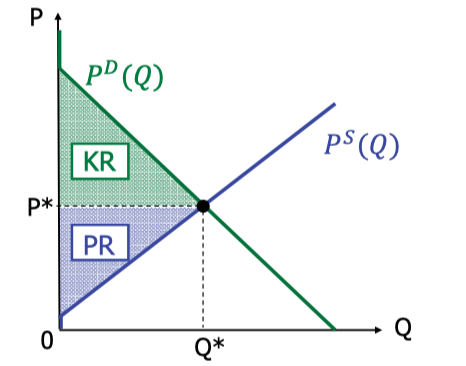
\includegraphics[scale=0.5]{img/krpr}
	\end{minipage}
\end{figure}  ~\smallskip

Die \textbf{Konsumentenrente} wird durch die Fläche oberhalb der inversen Angebotskurve beschrieben. Sie entspricht der Summe der Differenzen zwischen dem niedrigsten Betrag, für welche $x^*$ Einheiten des Gutes angeboten würden, und dem tatsächlichen Preis.  ~\newpage
		
\subsubsection*{Wohlfahrt und Wohlfahrtsverlust}

Die sogenannte Gesamtwohlfahrt ist die Summe aus Konsumenten-, Produzentenrente und möglicher Steuereinnahmen. Sie stellt den Nutzen des sich einstellenden Gleichgewicht dar. Ein Staatseingriff in den Markprozess, wie Höchst- oder Mindestpreise, Subvention und Besteuerung kann zu einem Wohlfahrtsverlust führen. Der Wohlfahrtsverlust ist demnach einfach die Differenz der Wohlfahrt vor und nach dem Eingriff. ~\bigskip

Im Fall der Einführung einer Steuer muss zwischen dem Preis der Nachfrager $p_D$ und dem Preis der Anbieter $p_S$ unterschieden werden. Insbesondere:
\begin{itemize}
	\item wird eine Mengensteuer eingeführt, wird für jede gekaufte Einheit ein Teil des Preises abgeführt. Die Anbieter erhalten lediglich den Verkaufspreis $p_D$ abzüglich der Steuerabgaben, das heißt $p_D = p_S + t$.
	\item wird eine Wertsteuer eingeführt, so wird für jede gekaufte Einheit ein  Anteil des Preises abgeführt. Die Anbieter erhalten lediglich einen um einen Faktor verringerten Verkaufspreis $p_D$, das heißt $p_D = (1 + \tau) \cdot p_S$.
\end{itemize} 
Analog können Subventionen auf die Menge und den Wert des Gutes \enquote{negative} Steuer aufgefasst werden. ~\bigskip

Allerdings muss trotz Steuer auf dem Markt weiterhin ein Gleichgewicht herrschen, das heißt
\begin{equation*}
	D(p^*_D) = S(p^*_S) \tag*{$(*)$}
\end{equation*} 

\begin{kr}[Wohlfahrtsverlust] ~\\
	Bei linearen Angebots- und Nachfragefunktionen können die Konsumenten- und Produzentenrenten, sowie die Steuereinnahmen und der DWL einfach über geometrische Gleichungen berechnet werden (Dreiecksflächen). ~\bigskip
	
	Zuerst ist aus diesem Grund das Gleichgewicht ohne Steuer zu berechnen und dies ergibt $p^*$ und $q*$. Danach mit Steuern berechnet man mittels $(*)$ das neue Gleichgewicht und erhält $p_D^*$ und $p_S^*$. Sei $p_{max}$ zusätzlich der Höchstpreis und $p_{min}$ der Mindestpreis (oft $= 0$) den die Nachfrage bereit ist zu zahlen. 
	
	\begin{minipage}[t]{0.25cm}
		~\
	\end{minipage}
	\begin{minipage}[t]{7.5cm}
		\vspace{0pt} ~\bigskip
		\begin{itemize}
			\item $KR = \frac{1}{2} \cdot (p_{max} - p_D^*) \cdot D(p_D^*)$
			\item $PR = \frac{1}{2} \cdot (p_{S}^* - p_{min}) \cdot D(p_D^*)$
			\item $Steuer = (p_D^* - p_S^*) \cdot D(p_D^*)$
			\item $DWL = \frac{1}{2} \cdot (p_D^* - p_S^*) \cdot (q^* - D(p_D^*))$
		\end{itemize}
	\end{minipage}
	\hspace{0.25cm}
	\begin{minipage}[t]{4.25cm}\vspace{0pt}
		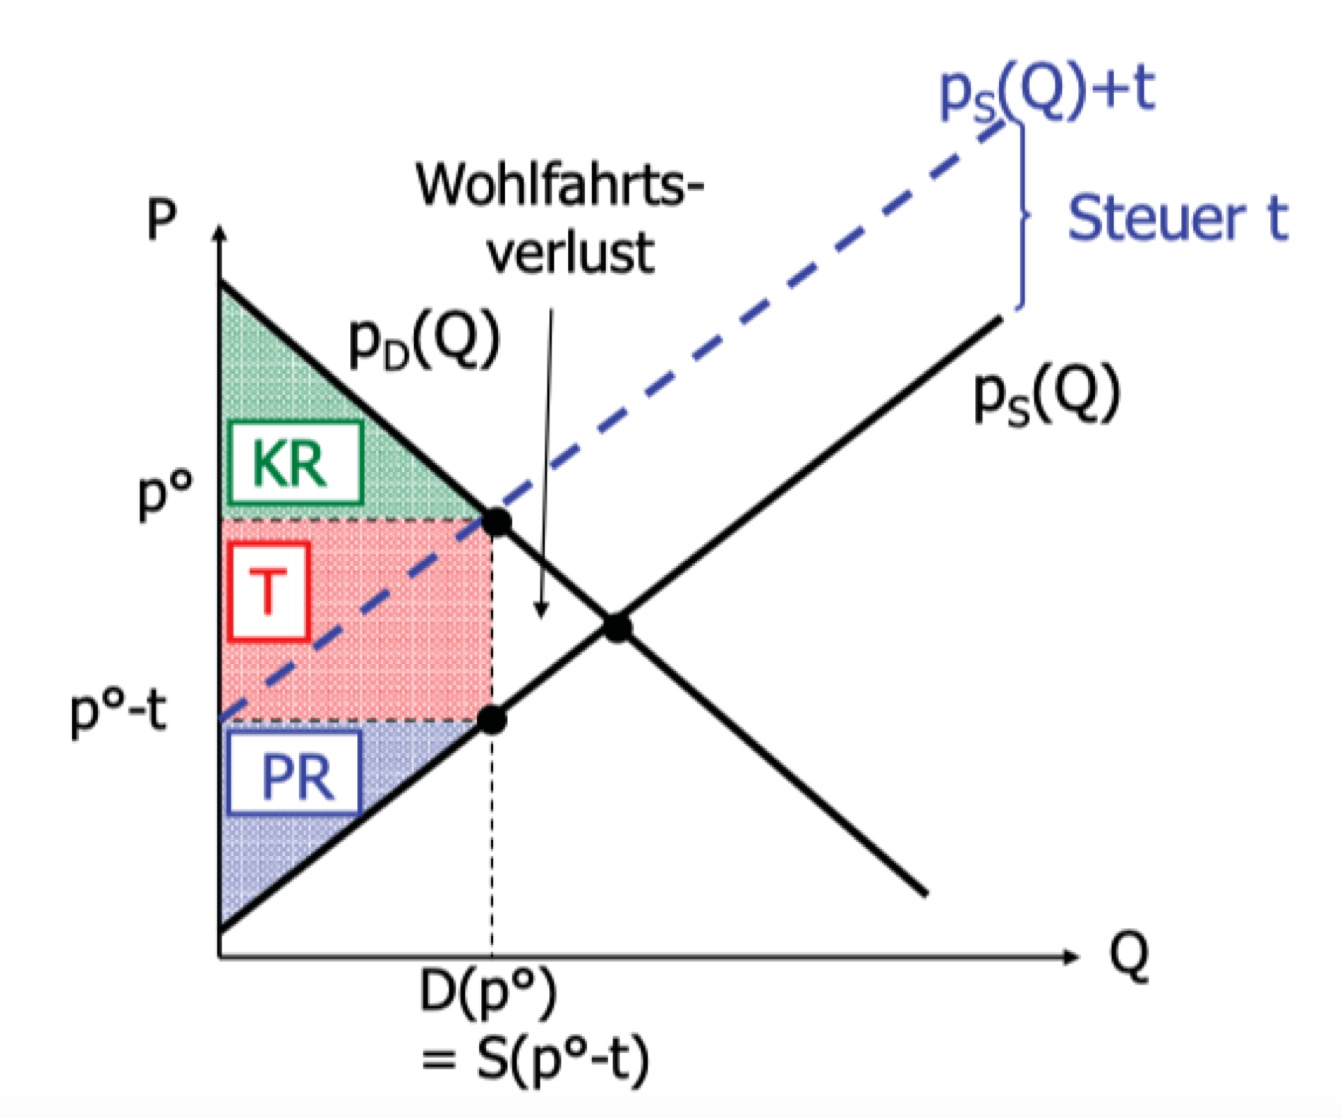
\includegraphics[scale=0.215]{img/dwl}
	\end{minipage}
\end{kr} ~\bigskip

In der Vorlesung wurde auch gezeigt, dass je weniger elastisch die Nachfrage (oder das Angebot) auf Preisänderungen reagieren, desto geringer ist die Zusatzlast durch eine Steuereinführung.
\chapter{Rational Choice}

\section{Präferenzen}

Ein \textbf{Güterbündel} ist eine vollständige Liste mit Mengenangaben für alle verfügbaren Güter. Mittels einer sogenannten \textbf{Präferenzordnung} können Güterbündel verglichen und damit Präferenzen ausdrückt werden. ~\bigskip

Für beliebige Güterbündel $x$ und $y$ führen wir die folgende Notation ein:
\begin{itemize}
	\item falls $x$ gegenüber $y$ strikt präferiert wird, dann $x \succ y$
	\item falls $x$ gegenüber $y$ schwach präferiert wird, dann $x \succeq y$
	\item falls der Konsument zwischen $x$ und $y$ indifferent ist, dann $x \sim y$
\end{itemize}

Präferenzordnungen sind allerdings nur ordinal und nicht kardinal. Wir können also nicht aussagen, \enquote{um wieviel besser} ein Bündel gegenüber einem anderen ist.

\subsubsection*{Die Axiome für Präferenzrelationen}

Folgende Eigenschaften können auf eine Präferenzordnung zutreffen:

\begin{itemize}
	\item \textbf{Vollständigkeit}: für jedes Paar verfügbarer Güterbündel $x$ und $y$ gilt entweder $x \succeq y$ oder $y \succeq y$. 
	\item \textbf{Reflexivität}: (dies folgt bereits aus Vollständigkeit) bei der Wahl zwischen zwei identischen Güterbündeln liegt keine strikte Präferenz vor: $x \succeq x$.
	\item \textbf{Transitivität}: für jede beliebige Auswahl von 3 Bündeln $x$, $y$ und $z$ soll gelten, dass aus $x \succeq y$ und $y \succeq z$ folgt, dass $x \succeq z$.
\end{itemize}

Eine Präferenzordnung die vollständig und transitiv ist, nennen wir Präferenzrelation. Häufig werden aber auch zusätzliche Eigenschaften gefordert:
\begin{itemize}
	\item \textbf{Strenge Monotonie}: Eine Präferenzrelation $\succeq$ ist streng monoton genau dann, wenn für alle Konsumpläne $x$ und $y$ gilt: wenn $x$ von jedem Gut mindestens so viel enthält wie $y$ und wenn $x$ von mindestens einem Gut echt mehr enthält als $y$, dann gilt $x \succ y$. 
	\item \textbf{Strenge Monotonie}: Eine Präferenzrelation $\succeq$ ist monoton genau dann, wenn für alle Konsumpläne $x$ und $y$ gilt: wenn $x$ von jedem Gut echt mehr enthält als $y$, dann gilt $x \succ y$. 
	\item \textbf{(Streng) konvexe Präferenzen}: Mischungen von indifferenten Konsumplänen sind (echt) bessre, als die der Mischung zugrundeliegenden Konsumpläne. Formal: wenn $x \tilde y$, dann gilt $\lambda x + (1 - \lambda) y \succeq (\succ) x$ für alle $\lambda \in [0, 1]$ ($\lambda \in (0, 1)$).
\end{itemize}

\subsubsection*{Indifferenzmenge}

Alle Konsumpläne, die nach einer Präferenzordnung indifferent (\enquote{genauso gut}) zu einem gegebenen Konsumplan $x$ sind, werden in der sogenannten Indifferenzmenge zu $x$ zusammengefasst:
$$ I(x) = \big\{ y \in X ~|~x \sim y \big\} $$
\begin{itemize}
	\item Wenn die Präferenzen transitiv sind, können sich zwei Indifferenzkurven nie schneiden.
	\item Jede Präferenzordnung lässt sich als ein System von Indifferenzkurven darstellen.
	\item Ist die Präferenzrelation streng monoton, so hat $I(x)$ eine negative Steigung
	\item Ist die Präferenzrelation streng monoton, so liegen \enquote{bessere Konsumpläne} auf höheren Indifferenzkurven, \enquote{schlechtere} auf niedrigeren.
\end{itemize}

Die Annahme die im folgenden stets getroffen wird, dass es nämlich lediglich zwei Güter gibt, ist keine richtige Einschränkung, da Gut 2 stets \enquote{alle anderen Güter} zusammenfassen kann.

\section{Theorie des Haushalts}

 Wir benötigen für die folgende Theorie diese Begriffe:

\begin{itemize}
	\item \textbf{Budgetbeschränkung}: die Ausgaben dürfen das Einkommen nicht überschreiten 
		$$ p_1 \cdot x_1 + p_2 \cdot x_2 \leq m. $$
	\item \textbf{Budgetmenge}: die Menge aller Konsumpläne die ein Konsument sich leisten kann 
		$$ B(m, p_1, p_2) = \big\{ (x_1, x_2) \in \mathbb{R}^2 ~|~p_1 \cdot x_1 + p_2 \cdot x_2 \leq m \big\}. $$
	\item \textbf{Budgetgerade}: oberer Rand der Budgetmenge
		$$ p_1 \cdot x_1 + p_2 \cdot x_2 = m $$ 
\end{itemize}

Hier sei angemerkt, dass $- \frac{p_1}{p_2}$ die Steigung der Budgetgerade ist. ~\bigskip

\subsubsection*{Komparative Statik der Budgetmenge}

Die Budgetmenge kann sich durch verschiedene Einflüsse ändern. Darunter fallen:
\begin{itemize}
	\item Einkommensveränderung, Pauschalsteuern und Pauschalsubventionen: führt zu einer Parallelverschiebung der Budgetgerade
	\item Veränderung des Preisverhältnisses $- \frac{p_1}{p_2}$ durch z.B. Mengen- oder Wertsteuern und Mengen- oder Wertsubventionen: führt zu einer Änderung der Steigung der Budgetgerade
	\item Rationierung: schneidet die Budgetmenge ab einer Menge ab
	\item Gleichmäßige Wertsteuer: ändern sich alle Preise im gleichen Verhältnis ist dies äquivalent zu einer Einkommensbesteuerung; somit verschiebt sich die Budgetgerade auch hier parallel
\end{itemize} 

% todo Während der Vorlesung: Bild zu Budgetmengen und deren Verschiebungen bzgl. Parametern

\subsubsection*{Unterschiedliche Präferenztypen}

\begin{itemize}
	\item \textbf{Perfekte Substitute}: bei perfekten Substituten ist der Konsum bezüglich jeder Mischung zweier indifferenter Konsumplänen wiederum indifferent. Die Indifferenzkurven sind im 2-Güter-Fall fallende Gerade. Sie sind streng monoton und konvex. Bsp.: Wasser und Säfte.
	\item \textbf{Perfekte Komplemente}: bei perfekten Komplementen möchte ein Konsument immer in einem bestimmten Verhältnis konsumieren (1:1 oder 3:2). Die Indifferenzkurven sind im 2-Güter-Fall L-förmig, sowie monoton und konvex. Die \enquote{Ecken} geben das optimale Konsumverhältnis an. Beispiel: rechte und linke Schuhe oder eine Tasse Tee und zwei Löffel Zucker.
	\item \textbf{Präferenzen mit Sättigungspunkt}: ein Sättigungspunkt (bliss point) ist ein Konsumplan, den der Konsument allen anderen Konsumplänen vorzieht. Dies verletzt das Axiom der Monotonie! Beispiel: Bier und Brezeln.
	\item \textbf{Neutrale Güter}: ein Gut ist für einen Konsumenten ein neutrales Gut, wenn seie Menge in einem Konsumklan keinen Einfluss auf die Beurteilung durch den Konsumenten hat. Die Indifferenzkurven sind parallel zur Achse des anderen Gutes.
	\item \textbf{Goods/Bads}: durch Erhöhen eines Goods wird das neue Güterbündel dem ursprünglichen gegenüber präferiert. Durch Erhöhen eines Bads wird das ursprünglichen Güterbündel dem neuen gegenüber präferiert. 
\end{itemize}

\section{Nutzentheorie}

Eine Nutzenfunktion $u(x)$ ordnet jedem Güterbündel einen Nutzen zu. Genau wie die Präferenzrelationen so sind Nutzenfunktionen lediglich ein ordinales Konzept. Ein Güterbündel $x$ wird genau dann $y$ bevorzugt, wenn $u(x) \geq u(y)$.

\subsubsection*{Repräsentationssatz}

Gegeben sei eine Präferenzrelation die vollständig, transitiv und stetig ist (d.h. jede stetige Präferenzrelation), so existiert eine Funktion, die sie repräsentiert. Ist andersherum eine Nutzenfunktion gegeben, die eine Präferenzrelation repräsentiert, so ist sie vollständig und transitiv.

\subsubsection*{Grenzrate der Substitution (MRS)}

Die Grenzrate der Substitution gibt das Tauschverhältnis an, zu dem ein Konsument Gut 1 gegeben Gut 2 tauschen würde. Dies entsprecht der Steigung der Indifferenzkurve.
	$$ MRS = - \frac{MU_1}{MU_2} = - \frac{\partial u(x_1, x_2)}{\partial x_1} \big/ \frac{\partial u(x_1, x_2)}{\partial x_2} $$ % todo Während der Vorlesung: Alternative Interpretation wäre, dass der Nutzen pro Preis gleich sein müsste
$MU_1$ bzw. $MU_2$ beschreiben den Grenznutzen von Gut 1 bzw. Gut 2 und sowohl die, als auch die MRS ist ein lokales Konzept.

\subsubsection*{Positiv monotone Transformation}

Da Nutzenfunktionen ein lediglich ordinales Konzept sind, können wir in gewissem Maß deren Wert verändern. Eine positiv monotone Transformation ist eine Funktion $v(x_1, x_2)$, falls
$$ v(x_1, x_2) = f(u(x_1, x_2)), $$
mit f' > 0. Typische Beispiele sind
\begin{itemize}
	\item Addition einer Konstanten: $v(x_1, x_2) = u(x_1, x_2) + c, c \in \mathbb{R}$
	\item Multiplikation mit einem positiven Faktor: $v(x_1, x_2) = a \cdot u(x_1, x_2), a \in \mathbb{R}^+$
	\item Positive Exponenten: $v(x_1, x_2) = \left(u(x_1, x_2) \right)^{z}, z \in \mathbb{R}^+$
\end{itemize}

Jede positiv monotone Transformation einer Nutzenfunktion stellt dieselbe Präferenzordnung dar wie die ursprüngliche Nutzenfunktion. Damit ändern positiv monotone Transformationen auch die MRS nicht (allerdings die Grenznutzen $MU_i$)!

\subsubsection*{Nutzenfunktion für bekannte Präferenzordnungen}
\begin{itemize}
	\item \textbf{Perfekte Substitute}: $u(x_1, x_2) = a \cdot x_1 + b \cdot x_2$, $a, b > 0$. Es gilt $MRS = - \frac{a}{b}$ und damit sind die Indifferenzkurven fallende Geraden.
	\item \textbf{Perfekte Komplemente}: $u(x_1, x_2) = \min \{ a \cdot x_1, b \cdot x_2 \}$, $a, b > 0$. Der Konsument möchte hier im festen Verhältnis $b : a$ konsumieren (in den \enquote{Ecken} der Indifferenzkurven). Die Optimalitätsbedingung ist damit: $a \cdot x_1 = b \cdot x_2$.
	\item \textbf{Cobb-Doublas Nutzenfunktion}: $u(x_1, x_2) = x_1^c \cdot x_2^d$, $c, d > 0$. Dies kann (und sollte) positiv monoton transformiert werden: sei $\alpha = \frac{c}{c + d}$
		$$ u(x_1, x_2) = x_1^{\alpha} \cdot x_2^{1 - \alpha}, \quad \alpha \in (0, 1) $$
		Für $x_1, x_2 > 0$ repräsentieren Cobb-Douglas Nutzenfunktionen streng monotone, streng konvexe Präferenzen. Es gibt hier immer eine optimale Entscheidung in einer innere Lösung (siehe \enquote{optimale Entscheidung})
	\item \textbf{Quasilineare Präferenzen}: $u(x_1, x_2) = v(x_1) + x_2$ mit $v' > 0$, $v'' < 0$. Die Indifferenzkurven sind \enquote{quasi parallel verschobene} Versionen voneinander.
\end{itemize}

\section{Optimale Entscheidung und Nachfrage}

Durch die Budgetmenge können wir beschreiben, was der Agent sich leisten kann. Durch Präferenzen wird ausgedrückt, was der Agent konsumieren möchte. Im folgenden kombinieren wir beide Konzepte und treffen bei gegebenen Preisen und gegebenem Einkommen $m$ in Abhängigkeit von den individuellen Präferenzen des Agenten eine optimale Konsumentscheidung. ~\bigskip

Die zentrale Frage ist also: welcher Konsumplan in der Budgetmenge maximiert den Nutzen des Konsumenten?
	$$ \max_{x_1, x_2 \in \mathbb{R}^+} u(x_1, x_2) ~\text{ s.t. }~ p_1 \cdot x_1 + p_2 \cdot x_2 \leq m $$ 
	
Der \textbf{optimale Konsumplan} ist der Konsumplan, unter allen die in der Budgetmenge liegen, der auf der höchsten Indifferenzkurve liegt. Bei monotonen Präferenzen liegt der optimale Konsumplan immer auf der Budgetgerade; damit suchen wir die Indifferenzkurve die im Allgemeinen gerade die Budgetgerade berührt und es gilt im Allgemeinen auch:
		$$ MRS \overset{!}{=} - \frac{p_1}{p_2}, $$
d.h. die Steigung der Indifferenzkurve = Steigung der Budgetgerade.
\begin{itemize}
	\item \enquote{Im Allgemeinen} da wir bereits gesehen haben, dass die MRS nicht immer bestimmbar sein muss (z.B. bei perfekten Komplementen), nicht-konvexe Nutzenfunktionen gegeben sein können oder eine Randlösung existiert. Wir werden deswegen im Folgenden das Vorgehen für verschiedene Präferenzordnungen genauer betrachten.
	\item Intuitiv wird durch diese Bedingung gefordert, dass von beiden Gütern der gleiche Grenznutzen im Verhältnis zum Preis erbracht wird, da $\frac{MU_1}{p_1} = \frac{MU_2}{p_2}$.
\end{itemize}

\begin{kr}[Optimalität] ~\
	\begin{itemize}
		\item \textbf{Perfekte Komplemente}: $u(x_1, x_2) = \min \{ a \cdot x_1, b \cdot x_2 \}$. Das Optimum liegt immer an der Ecke der Indifferenzkurve, unabhängig vom Preisverhältnis. Die Nutzenfunktion gibt das Optimum $a \cdot x_1 = b \cdot x_2$ vor. Wir lösen diese Gleichung nach $x_1$ oder $x_2$ auf und setzen dies in die Budgetgerade ein.
		\item \textbf{Perfekte Substitute}: $u(x_1, x_2) = a \cdot x_1 + b \cdot x_2$. Die Steigung der Indifferenzkurve ist konstant und damit ist $MRS = - \frac{a}{b}$. Es können nun drei mögliche Fälle eintreten:
			\begin{itemize}
				\item die Budgetgerade verläuft steiler als die Indifferenzkurven: 
					$$ \big| - \frac{a}{b} \big| < \big| - \frac{p_1}{p_2} \big| $$
					$\Rightarrow$ Randlösung: es wird nur $x_2$ konsumiert, d.h. $x^* = (0, \frac{m}{p_2})$.
				\item die Budgetgerade verläuft flacher als die Indifferenzkurven: 
					$$ \big| - \frac{a}{b} \big| > \big| - \frac{p_1}{p_2} \big| $$
					$\Rightarrow$ Randlösung: es wird nur $x_1$ konsumiert, d.h. $x^* = (\frac{m}{p_1}, 0)$.
				\item Falls Budgetgerade und Indifferenzkurven dieselbe Steigung haben, d.h. 
					$$ \big| - \frac{a}{b} \big| = \big| - \frac{p_1}{p_2} \big| $$
					sind alle Güter auf der Budgetgerade optimal.
			\end{itemize}
		\item \textbf{Cobb-Douglas}: $u(x_1, x_2) = x_1^c \cdot x_2^d$, $c, d > 0$. Bei Cobb-Douglas Nutzenfunktionen gibt es immer eine innere Lösung. Man kann hier die Gleichung
			$$ MRS = - \frac{p_1}{p_2}, $$
			lösen und das Ergebnis in die Budgetgerade einsetzen. Der einfachere Weg ist allerdings die Nutzenfunktion positiv monoton zu transformieren, sodass mit $\alpha = \frac{c}{c + d}$
				$$ u(x_1, x_2) = x_1^{\alpha} \cdot x_2^{1 - \alpha}, \quad \alpha \in (0, 1) $$
			gilt. Das Optimum lässt sich dann direkt über die folgende Formel bestimmen:
			$$ x^* = \left( \frac{\alpha m}{p_1}, \frac{(1 - \alpha) m}{p_2} \right) $$
		\item \textbf{Quasilineare Präferenzen}: $u(x_1, x_2) = v(x_1) + x_2$ mit $v' > 0$, $v'' < 0$. Durch die besondere Form der Indifferenzkurven möchte man unabhängig vom Einkommen immer dieselbe Menge von Gut 1 konsumieren (falls die Nutzenfunktion linear in $x_2$ ist). Dies ist nur möglich, wenn das Einkommen $m$ dafür ausreicht und damit ei \enquote{kritisches Einkommen} $m^{krit}$ nicht unterschreitet:
			\begin{itemize}
				\item Bestimme $x_1^{krit}$ über die Optimalitätsbedingung $MRS = - \frac{p_1}{p_2}$
				\item Berechne kritisches Einkommen $m^{krit} = p_1 \cdot x_1^{krit}$. 
				\item Für $m > m^{krit}$: $x_1^* = x_1^{krit}$, $x_2^* = \frac{m - p_1 \cdot x_1^{krit}}{p_2}$
				\item Für $m \leq m^{krit}$: $x^* = (\frac{m}{p_1}, 0)$
			\end{itemize}
	\end{itemize}	
\end{kr}

\chapter{Nachfrageanalyse}

Ist eine optimale Entscheidung getroffen, ist die nächstgelegene Frage, wie sich diese Entscheidung abhängig von Parametern ändert. ~\bigskip

Nachfrageänderung aufgrund einer Einkommensänderung:
\begin{itemize}
	\item \textbf{Normale Güter}: die nachgefragte Menge steigt nach einem Einkommensanstieg und fällt nach einem Einkommensabfall ($\frac{\Delta x_i}{\Delta m} > 0$).
	\item \textbf{Inferiore Güter}: die nachgefragte Menge sinkt nach einem Einkommensanstieg und steigt nach einem Einkommensabfall ($\frac{\Delta x_i}{\Delta m} < 0$).
\end{itemize}

Nachfrageänderung aufgrund der Preisänderung eines Gutes:
\begin{itemize}
	\item \textbf{Gewöhnliche Güter}: die nachgefragte Menge sinkt nach einer Preiserhöhung und steigt nach einer Preissenkung ($\frac{\Delta x_i}{\Delta p_i} < 0$).
	\item \textbf{Giffen Güter}: die nachgefragte Menge steigt nach einer Preiserhöhung und sinkt nach einer Preissenkung ($\frac{\Delta x_i}{\Delta p_i} > 0$).
\end{itemize}

\section{Komperative Statistik der Nachfrage}

Wie ändert sich die Nachfrage nach einem Gut aufgrund von Einkommens- und Preisänderungen.

\subsubsection*{Auswirkung einer Einkommensänderung auf die Nachfrage bei konstanten Preisen}

\begin{itemize}
	\item \textbf{Einkommensexpansionspfad (EEP)}
		\begin{itemize}
			\item Verbindung aller optimalen Konsumpläne in Abhängigkeit vom Einkommen $m$ im $(x_1, x_2)$-Diagramm.
			\item Grafisch bestimmt man den EEP durch Parallelverschiebung der Budgetgeraden.
		\end{itemize} % todo Zeichnung EEP für normale Güter
	\item \textbf{Engelkurve}
		\begin{itemize}
			\item Abbildung der Änderung der Nachfrage eines Gutes $x_i$ (bei Einkommensänderung) im $(x_i, m)$-Diagramm
			\item Die Änderung der nachgefragten Menge des anderen Gutes $x_j$ wird nicht explizit abgebildet.
		\end{itemize} % todo Zeichnungen
\end{itemize}

\subsubsection*{Auswirkung einer Eigenpreisänderung auf die Nachfrage des Gutes bei konstanten restlichen Preisen und gegebenem Einkommen}

\begin{itemize} \setcounter{enumi}{2}
	\item \textbf{Preisexpansionspfad (PEP)}
		\begin{itemize}
			\item Bildet ab, wie sich der optimale Konsumplan nach einer Preisänderung anpasst
			\item Grafisch im $(x_1, x_2)$-Diagramm durch Drehung der Budgetgerade im Punkt $\frac{m}{p_j}$.
		\end{itemize}
	\item \textbf{Nachfragekurve}
		\begin{itemize}
			\item Abbildung der Änderung der Änderung der Nachfrage eines Gutes $x_i$ im $(x_i, p_i)$-Diagramm
			\item Die Änderung der nachgefragten Menge des anderen Gutes $x_j$ wird nicht explizit abgebildet
		\end{itemize}	
\end{itemize}

EEP, Engelkurve, PEP und Nachfragekurve sehen für unterschiedliche Nachfragefunktionen bzw. Präferenzordnungen unterschiedlich aus. Wenn sich allerdings alle Preise und das Einkommen simultan um denselben Faktor ändern, ändert sich die Nachfrage nicht.

\subsubsection*{Auswirkung einer Fremdpreisänderung auf die Nachfrage eines Gutes bei konstantem Eigenpreis und gegebenem Einkommen}

\begin{itemize}
	\item \textbf{Substitute}: Güter bei denen, falls ein Gut teurer wird, sich der  Konsument bemüht, dieses Gut durch sein Substitut zu ersetzen ($\frac{\Delta x_i}{\Delta p_j} > 0$)
	\item \textbf{Komplemente}: Güter bei denen, falls ein Gut teurer wird, der Konsument weniger davon nachfragen wird und auch den Konsum der komplementären Güter einschränkt ($\frac{\Delta x_i}{\Delta p_j} < 0$)
\end{itemize}
% todo Zeichnungen
\section{Stusky-Zerlegung}

Eine Veränderung des Preises eines Guts (z.B. $p_1$ sinkt auf $p_1'$) hat zwei Effekte auf die Nachfrage:
\begin{itemize}
	\item Die Budgetmenge wird größer, wodurch die Kaufkraft steigt. Die allein daraus resultierende Änderung der Nachfrage = Einkommenseffekt.
	\item Das Preisverhältnis $\frac{p_1}{p_2}$ ändert sich, wodurch die Budgetgerade flacher wird. Die hieraus  resultierende Änderung der Nachrage bei konstanter Kaufkraft = Substitutionseffekt
\end{itemize}

\subsubsection*{Gesamteffekt der Preisänderung}

Durch die Preisänderung ändert sich die Nachfrage, was wir im Gesamteffekt festhalten:
	$$ \Delta x_1^{GE} = x_1^{*}(p_1', p_2, m) - x_1^*(p_1, p_2, m) $$
	
\subsubsection*{Substitutionseffekt}

$$ \Delta x_1^{s} = x_1^*(p_1', p_2, m') - x_1^*(p_1, p_2, m) $$

\begin{itemize}
	\item Nachfrageänderung aufgrund Änderung des relativen Preisverhältnisses
	\item Kaufkraft wird konstant gehalten (altes optimales Güterbündel $x^*$ liegt auf der Budgetgeraden), wodurch wird ein hypothetisches Einkommen $m'$ einführen müssen:
		$$ m' = \Delta m + m ~\text{ mit } ~\Delta m = x_1^* \cdot \Delta p_1 = x_1^* \cdot (p_1' - p_1)  $$
	\item Die Nachfrageänderung aufgrund des Substitutionseffekts ist immer entgegengesetzt der auslösenden Preisänderung (auch bei Giffen-Gütern!)
\end{itemize}

\subsubsection*{Einkommenseffekt}

$$ \Delta x_1^{n} = x_1^{*}(p_1', p_2, m) - x_1^*(p_1', p_2, m') $$

\begin{itemize}
	\item Nachfrageänderung aufgrund der Änderung der Kaufkraft (relatives Preisverhältnis konstant)
\end{itemize}

\begin{kr}[Stusky-Zerlegung] ~\
	Zur Berechnung der Effekte benötigen wir:
	\begin{itemize}
		\item $x_1^*(p_1, p_2, m)$: optimales Bündel vor der Preisänderung
		\item $x_1^*(p_1', p_2, m')$: optimales Bündel bei neuen Preisen und fiktivem Einkommen $m'$
		\item $x_1^*(p_1', p_2, m)$: optimales Bündel nach Preisänderung
	\end{itemize}
	Dann ist
	\begin{itemize}
		\item Substitutionseffekt: $\Delta x_1^{s} = x_1^*(p_1', p_2, m') - x_1^*(p_1, p_2, m)$
		\item Einkommenseffekt: $\Delta x_1^{n} = x_1^{*}(p_1', p_2, m) - x_1^*(p_1', p_2, m')$
		\item Gesamteffekt: $\Delta x_1^{GE} = \Delta x_1^{s} + \Delta x_1^{n}$.
	\end{itemize}
\end{kr}

% todo Bild

\subsubsection*{Nachfragefunktion und Totale Variation}

Eine Funktion $f(x_1 ,x_2, \dotsc, x_n)$ ist \textbf{homogen} vom Grade $r$, genau dann, wenn:
$$ z^r \cdot f(x_1, x_2, \dotsc, x_n) = f(z \cdot x_1, z \cdot x_2, \dotsc, z \cdot x_n) \quad \text{(für alle $z > 0$)} $$
Nachfragekurven bzw. Budgetmengen sind homogen vom Grad 0; das liegt daran, dass:
\begin{align*}
	B(z \cdot p, z \cdot m) & = \{ x \in X ~|~ x \geq 0, z \cdot p_1 + z \cdot p_2 + \dotsc + z \cdot p_n \leq z \cdot m \} \\
	& = \{ x \in X ~|~ x \geq 0, p_1 + p_2 + \dotsc + p_n \leq m \} = B(p, m)
\end{align*}
Daraus folgt, dass da proportionale Anpassungen die Budgetmenge unverändert lassen, die Nachfragekurve als Lösung des Nutzenmaximierungsproblems invariant gegenüber proportionalen Änderungen aller Preise $p$ und des Einkommens $m$ ist. 
% todo Während der Vorlesung: Was hat dieses Ergebnis mit Inflation zu tun?

\subsubsection*{Slutsky-Zerlegung nach Hicks}

Analog zur obigen Slutsky-Zerlegung ist auch hier eine Preisveränderung der Ausgangspunkt. Angenommen der Preis $p_1$ fällt auf $p_1'$, so resultiert erneut eine Nachfrageveränderung. Die Idee von Hicks ist allerdings die Aufspaltung in Einkommens- und Substitutionseffekt auf einen anderen Grundgedanken zu stützen. ~\bigskip

Slutsky hat ein fiktives Einkommen $m'$ eingeführt, dass die Kaufkraft konstant hält; der Nutzer soll sich auch bei den neuen Preisen das alte Güterbündel leisten können. Bei Hicks wird allerdings ein Einkommen eingeführt, sodass der ursprüngliche Nutzen optimal bleibt. ~\bigskip % todo Während der Vorlesung: Zeichnungen zur Erklärung

Auch hier ist im Substitutionseffekt die Änderungen des Preises stets entgegengesetzt der nachgefragten Menge, d.h. Preis und nachgefragte Menge haben entgegengesetzte Vorzeichen, also: % todo Während der Vorlesung: WARP beim Beweis!

$$ \frac{\Delta x_i^s}{\Delta p_i} < 0 $$

Bei kleinen Preisänderungen sind die  Substitutionseffekte nach Slutsky und Hicks gleich.
\chapter{Theorie der Unternehmung}
% todo Insbesondere ist zu überprüfen, ob sich nicht-produzieren lohnt!
Wir betrachten Unternehmen bzw. Firmen als Einrichtungen, die Inputs $x$ in Outputs $y$ transformieren.
\begin{figure}[htbp!]
	\begin{minipage}[t]{8cm} \vspace{0pt} ~\medskip
	
		 Die technischen Möglichkeiten einer Unternehmung sind durch die realisierbaren Input-Output-Kombinationen beschrieben, ihre Technologiemenge.
	\end{minipage}
	\hspace{0.25cm}
	\begin{minipage}[t]{4cm}\vspace{0.01pt}
		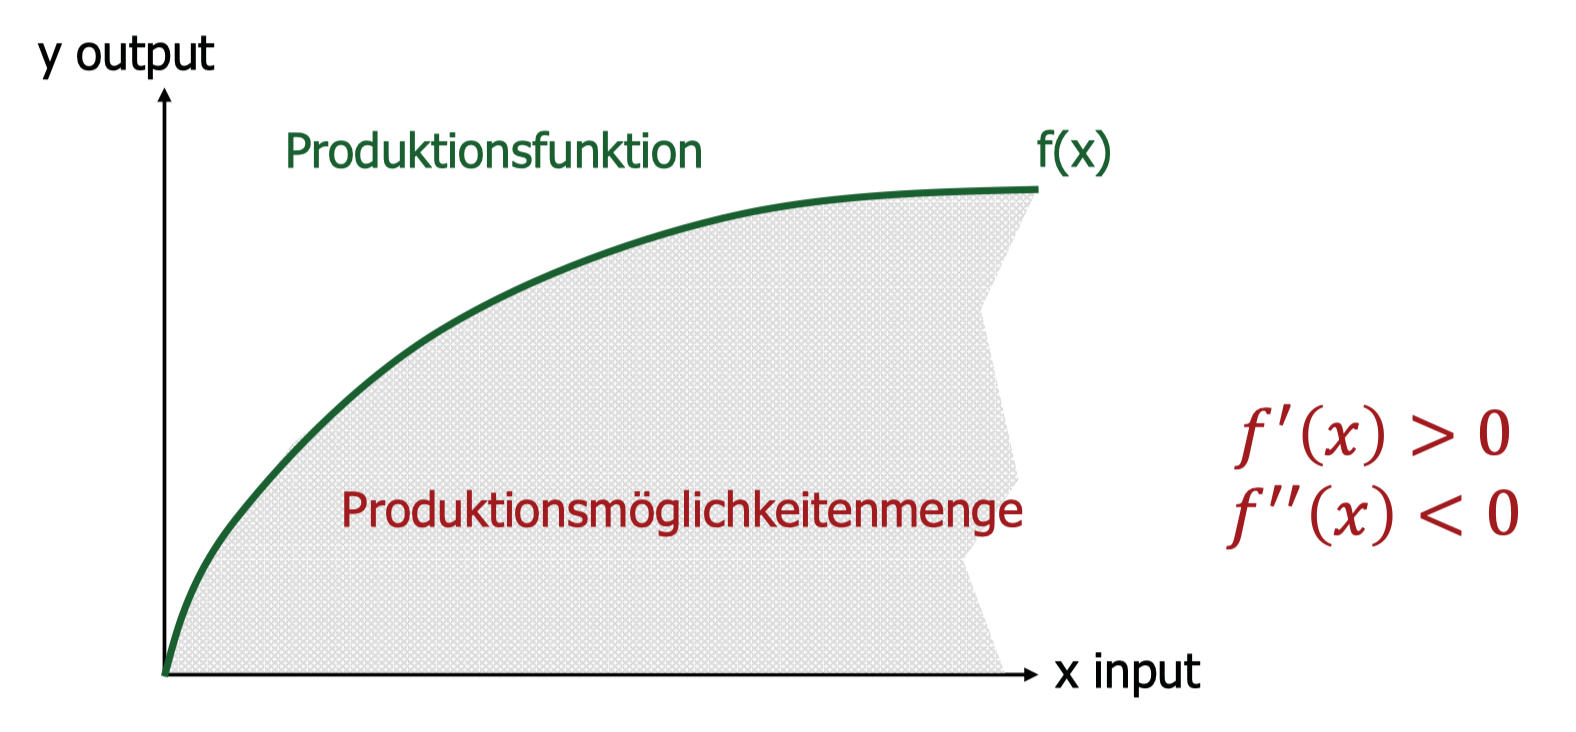
\includegraphics[scale=0.225]{img/technologiemenge}
	\end{minipage}
\end{figure} 

Eine Produktion ist \textbf{technisch effizient}, wenn ein vorgegebener Output mit geringst möglichen Inputmengen hergestellt wird. Analog ist eine Allokation technisch effizient, wenn es nicht möglich ist, die Produktionsmenge (PM) eines Gutes zu erhöhen, ohne gleichzeitig die PM eines anderen Gutes zu reduzieren.

\begin{itemize}
	\item effiziente Produktionspläne liegen auf dem Rand der Technologiemenge. Dieser Rand wird durch die Produktionsfunktion beschrieben. Diese gibt für jede Menge an Inputs die maximal mögliche Outputmenge an: $y = f(x_1, \dotsc, x_n)$
\end{itemize}

Wir nennen
\begin{itemize}
	\item eine Technologie \textbf{monoton}, wenn eine Inputerhöhung, zu keiner Outputverringerung führt ($\frac{\partial f}{\partial x_i} \geq 0$).
	\item eine Technologie \textbf{konvex}, wenn für beliebige Inputkombinationen $z$ and $x$, mit $y = f(z) = f(x)$, gilt, dass deren Mischung $\lambda z + (1-\lambda) x$ mindestens $y$ Outputeinheiten erzeugt werden, d.h. $f(\lambda z + (1-\lambda)x) \geq y$, $(0 < \lambda < 1)$.
\end{itemize}

Bei der Optimierung können zwei Fälle auftreten. Von einer Betrachtung in der kurzen Frist wird dann gesprochen, wenn mindestens ein Produktionsfaktor nicht unmittelbar angepasst werden kann, also fix ist. Hier muss lediglich die Gewinnfunktion nach dem verbleibenden Faktor maximiert werden:

$$ \max_{x_1} p f(x_1, \overline{x_2}) - w_1 x_1 - \underbrace{w_2 \overline{x_2}}_{\text{Fixkosten}} $$

Langfristig Frist können alle allerdings alle Produktionsfaktoren angepasst werden und die Optimierung ist etwas komplizierter.

\subsubsection*{Grenzprodukte der Inputfaktoren}

Das Grenzprodukt eines Inputfaktors $i$ gibt an, um wieviel der Output $y$ steigt, wenn die Einsatzmenge des Faktors $i$ geringfügig erhöht wird.
$$ MP_i = \frac{\partial f(x_1, x_2)}{\partial x_i} \geq 0 $$

\subsubsection*{Isoquanten und TRS}

Analog zu Indifferenzkurven sind Isoquanten alle technisch effizienten Inputkombinationen die zu gleichem Output führen. Die (negative) Steigung der Isoquanten ist die Technische Rate der Substitution. Sie gibt das Verhältnis an, in dem Input 2 durch Input 1 bei konstanten Output substituiert werden kann.
$$ TRS = - \frac{MP_1}{MP_2} = - \frac{\partial f(x_1, x_2)}{\partial x_1} \big/ \frac{\partial f(x_1, x_2)}{\partial x_2} $$
% todo beispiel

Achtung! Produktionsfunktionen kann man nicht positiv monoton transformieren, da sie kein rein ordinales Konzept wie die Nutzenfunktionen sind.

Außerdem ist zu beachten, dass oft es zunehmend schwieriger wird einen der Produktionsfaktor durch einen anderen bei konstantem Output zu substituieren. Dies wird als abnehmende Technische Rate der Substitution (im Absolutwert) bezeichnet.

\begin{figure*}[!htbp] \centering
	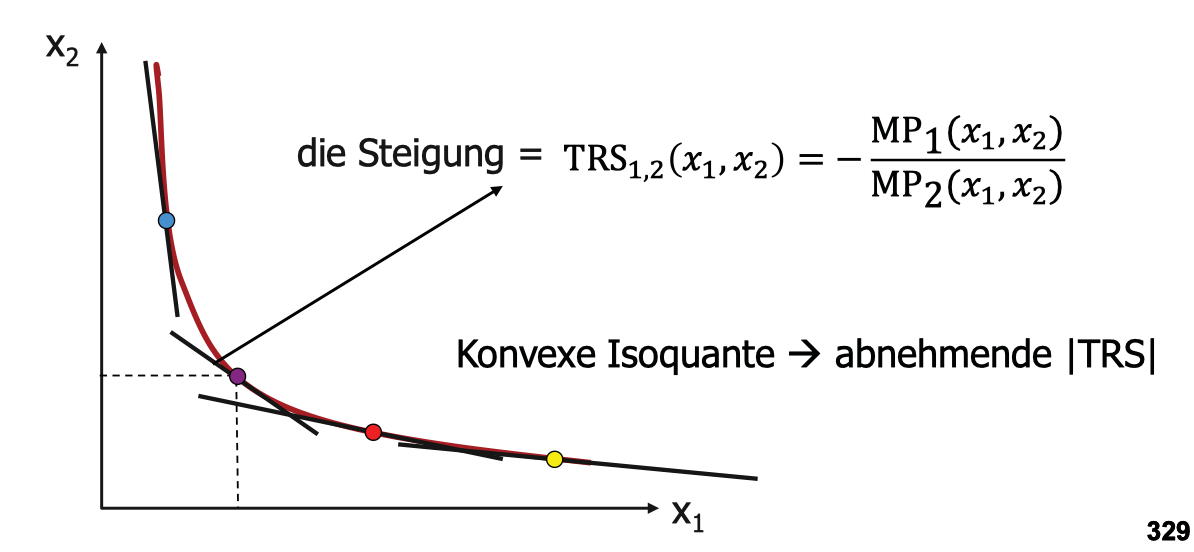
\includegraphics[scale=0.4]{img/trs}
\end{figure*}

% klassische vs neoklassische Produktionsfunktion

\subsubsection*{Skalenerträge}
Gegeben: $f(x_1, x_2)$. Wie verhält sich die Output-Menge bei Ver-t-fachung aller Inputgüter?
\begin{description}
	\item[\hspace{0.5cm}1. Fall:] $f( t \cdot x_1, t \cdot x_2) < t \cdot f(x_1, x_2)$: fallende Skalenerträge 
	\item[\hspace{0.5cm}2. Fall:] $f( t \cdot x_1, t \cdot x_2) = t \cdot f(x_1, x_2)$: kostante Skalenerträge 
	\item[\hspace{0.5cm}3. Fall:] $f( t \cdot x_1, t \cdot x_2) > t \cdot f(x_1, x_2)$: steigende Skalenerträge 	
\end{description}

\section{Gewinnmaximierung}

Es bleibt auch hier die zentrale Verhaltensannahme bestehen: alle Unternehmen maximieren ihren Gewinn. Dabei ist der Erlös eines Unternehmens das Produkt aus der verkauften Menge und dem Preis für den Output. Seien $x_1$ bzw. $x_2$ die eingesetzten Input-Mengen (zur Produktion der Output-Menge $y$) sowie $w_1, w_2$ die Faktorinputpreise von Faktor 1 und 2. Es ergibt sich das \textbf{Gewinnmaximierungsproblem}:
$$ \max \Pi(x_1, x_2) = p \cdot f(x_1, x_2) - (w_1 \cdot x_1 + w_2 \cdot x_2) $$
Dabei seien 
\begin{itemize}
	\item \textbf{Erlösfunktion}: $R(x_1, x_2) = p \cdot y = p \cdot f(x_1, x_2)$; deren Ableitung ist der Grenzerlös $MR$.
	\item \textbf{Kostenfunktion}: $C(x_1, x_2, w_1, w_2) = w_1 \cdot x_1 + w_2 \cdot x_2$; deren Ableitung sind die Grenzkosten $MC$.
\end{itemize}
Im Gewinnmaximum muss durch das Gewinnmaximierungsproblem im Allgemeinen gelten, dass 
$$ TRS = - \frac{w_1}{w_1} $$
Die Lösung dieser Gleichung ergibt die \textbf{bedingten Faktornachfragen} $x_1^*(p, w_1, w_2)$ und $x_2^*(p, w_1, w_2)$. Diese geben an, welche Inputmengen ein Unternehmen nachfragen muss, um seinen Gewinn zu maximieren. Auch die bedingten Faktornachfragen sind invariant gegenüber proportionalen Anstiegen (z.B. Verdopplung) von Faktorpreisen (obwohl die Produktionskosten reagieren).

\section{Kostenminimierung}

Setzt man die bedingten Faktornachfragen in die Kostenfunktion ein, so erhält man eine Funktion die die Minimalkosten für die Produktionsmenge $y$ angibt:
	$$ C(y) = C(w_1, w_2, y) = w_1 x_1^* + w_2 x_2^* $$
Auch lassen sich die Skalenerträge von Kostenfunktionen untersuchen:
\begin{itemize}
	\item \textbf{Konstante Skalenerträge}: $C(w, y) = y \cdot C(w, y = 1)$. 
	\item \textbf{Steigende Skalenerträge}: $C(w, y) > y \cdot C(w, y = 1)$.
	\item \textbf{Fallende Skalenerträge}: $C(w, y) < y \cdot C(w, y = 1)$
\end{itemize}

Im Allgemeinen lassen sich die Kosten in zwei Teile aufteilen:
\begin{itemize}
	\item \textbf{Fixkosten} $F$: All Kosten, die unabhängig von der Produktionsmenge $y$ entstehen. Beispiel: Miete.
	\item \textbf{Variable Kosten} $C_v(y)$: Alle Kosten, die sich mit der Produktionsmenge $y$ verändern. Beispiel: Rohstoffe.
\end{itemize}

Für die folgenden Betrachtungen benötigen wir ein paar zusätzliche Begriffe:
\begin{itemize}
	\item \textbf{Grenzkosten} $MC(y)$: die Grenzkosten sind \enquote{zusätzlichen Kosten}, die durch die Produktion \enquote{einer zusätzlichen Outputeinheit} entstehen. Formal sind die Grenzkosten also die erste Ableitung der Kostenfunktion nach $y$: $C'(y)$.
	\item \textbf{Durchschnittskosten} $AC$: die Produktionskosten, die durchschnittlich auf eine einzelne Outputeinheit bei der Produktion von insgesamt $y$ Einheiten entfallen, werden als Durchschnittskosten bzw. Stückkosten bezeichnet. Formale Definition: $AC(y) = \frac{C(y)}{y}$.
	\item Analog lassen sich die durchschnittlichen Fixkosten $AFC$ und die durchschnittlichen variable Kosten $AVC$ definieren und es gilt: $AC(y) = AFC(y) + AVC(y)$.
\end{itemize}

\begin{figure*}[!htbp] \centering
	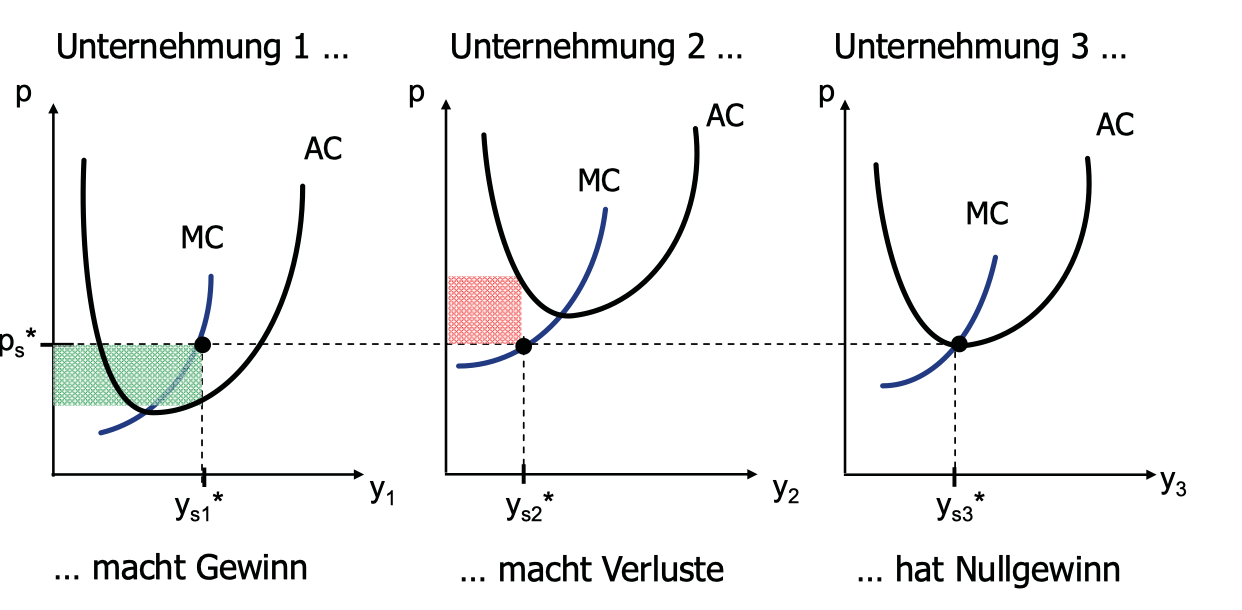
\includegraphics[scale=0.2425]{img/acmc}
\end{figure*}

Es gilt: die Grenzkostenkurve ($MC$-Kurve) schneidet die Durschnittskostenkurve ($AC$-Kurve) in ihrem Minimum.
\chapter{Marktformen und vollkommener Wettbewerb}

Wenn neue Unternehmen in eine Branche eintreten, steigt das Angebot, wodurch die (inverse) Angebotskurve flacher wird. Daraus folgt, dass der Gleichgewichtspreis sinkt und sich der Gewinn verringert. Wenn andererseits Unternehmen aus dem Markt austreten, wird die (inverse) Angebotskurve steiler. ~\smallskip

Kurzfristig kann es sowohl zu ökonomischen Gewinnen oder ökonomischen Verlusten kommen. Sobald jedoch eine Firma Verluste schreibt, so muss sie sich zwischen einem Shutdown und einem Marktaustritt entscheiden.
\begin{itemize}
	\item Die Entscheidung die Produktion temporär einzustellen (\textbf{Shutdown}), $y = 0$ ist eine Entscheidung hinsichtlich der kurven Frist. Dies tritt ein, falls $p < AVC$.
	\item Falls der Preis langfristig unter den Durchschnittskosten bleibt, ist es für eine Unternehmung zur Vermeidung permanenter Verlust optimal, aus dem Markt auszutreten (\textbf{Marktaustritt}). Dies tritt ein, falls $p < AC$.
\end{itemize}

In einer positiven ökonomischen Gewinne  treten neue Unternehmen in den Markt ein, so dass die Angebotskurve flacher wird. Daraus folgt, dass der Gleichgewichtspreis sinkt und sich der Gewinn verringert.

\subsubsection*{Vollkommener Wettbewerb}

Eine Situation in der alle Anbieter als Preisnehmer agieren und lediglich über ihre Angebotsmenge entscheiden, nennt man vollkommener Wettbewerb (z.B. unbegrenzte Markteintritte). Jeder Anbieter maximiert dann seinen Gewinn bezüglich $y$:
	$$ \max_y \Pi(y) = R(y) - C(y) = p \cdot y - C(y) $$
	
\begin{itemize}
	\item \textbf{Marginal Revenue}: Der Grenzerlös $MR(y)$ ist die erste Ableitung der Erlösfunktion $R(y)$.
	\item \textbf{Marginal Costs}: Die Grenzkosten $MC(y)$ sind die erste Ableitung der Kostenfunktion $C(y)$
	\item Im Gewinnmaximum gilt nach Bedingung erster Ordnung demnach: Grenzerlös = Grenzkosten ($MR = MC$)
\end{itemize}

Ein Unternehmen bietet bei vollständiger Konkurrenz somit bei jedem Preis diejenige Menge an, bei der die Grenzkosten dem gegebenem Preis entsprechen. Dies ist die gewinnmaximierende Outputmenge.

\begin{kr}[Unternehmungen im vollkommenen Wettbewerb]
	Da bei vollkommendem Wettbewerb die Anbieter als Preisnehmer agieren, muss im Optimum gelten:
	$$ MC(y) = p(y) $$
	Auflösen dieser Gleichung nach $y$ ergibt die optimale Produktionsmenge.
\end{kr} % todo \subsubsection*{Langfristiges Marktgleichgewicht}


\chapter{Monopol}

Wenn die Angebotsentscheidung eines einzelnen Anbieters den Marktpreis beeinfluss, dann hat dieser Anbieter \textbf{Marktmacht}. Insbesondere ein Monopolist besitzt Marktmacht. ~\bigskip

Ein Monopolist ist der einzige Anbieter in einem Markt. Er kann entweder den Preis oder die Menge festlegen, die jeweils andere Variable wird durch die gegebene Marktnachfragefunktion bestimmt. Ein Monopolist kann dabei durch Verknappung des Angebots den Preis in die Höhe treiben, sodass ein Preis erreicht wird, der über den Grenzkosten liegt. Durch die mögliche Preiserhöhung in dieser Situation kann ein Wohlfahrtsverlust entstehen.

\subsubsection*{Gewinnmaximierungsproblem des Monopolisten}
$$\max \Pi(y) = R(y) - C(y) = p(y) \cdot y - C(y)$$
\begin{itemize}
	\item Im Monopol-Optimum gilt: $MR = MC$ (Grenzerlös = Grenzkosten). Erlös und Kostenfunktion haben also in diesem Punkt dieselbe Steigung.
	\item Wäre nämlich der zusätzliche Erlös (Grenzerlös) bei einer Erhöhung des Outputs größer als die zusätzlichen Kosten (Grenzkosten), dann könnte der Gewinn erhöht werden, indem man eine zusätzliche Outputeinheit herstellt. Analog für den anderen Fall.
	\item Ein gewinnmaximierender Monopolist wird immer im elastischen Bereich der Nachfrage $(|\epsilon_D(p)| \geq 1$) anbieten. Dies kann man unter gewissen Bedingungen aus der sogenannten Amoroso-Robinson-Gleichung ablesen: $p(y) \cdot \left[ 1 - \frac{1}{|\epsilon|} \right] = MC(y)$
	\item Die Höhe des monopolistischen Preisaufschlags hängt somit von der Preiselastizität der Nachfragefunktion ab: je elastischer die Nachfrage, umso geringer der Preisaufschlag. Im Fall einer unendlich elastischen Nachfrage sind Monopol- und Wettbewerbspreis gleich. 
\end{itemize} 

\begin{kr}[Monopolist]
	Um die optimale Ausbringungsmenge $y*$ zu ermitteln, lösen wir das Problem:
	$$ \max \Pi(y) = p(y) \cdot y - C(y) $$
	was zur folgenden Gleichung führt:
		$$ p(\hat{y}) + p'(\hat{y}) \cdot y = MC(\hat{y}) $$	
	Da der Monopolist die Option hat nicht zu produzieren, müssen wir überprüfen, ob sich dies lohnen würde. Ist $\Pi(\hat{y}) > \pi(0)$, so ist $y^* = \hat{y}$ und ansonsten $y^* = 0$.
\end{kr}
\chapter{Oligopol}

Ein Oligopol ist ein markt mit wenigen aktiven Anbieter, die alle über Marktmacht verfügen. Ein Oligopol ist somit eine Art \enquote{Mischform} zwischen dem Monopol und dem vollkommenen Wettbewerb. Wir betrachten vereinfachend den Fall des Duopols mit 2 identischen Anbietern. Der Output des Unternehmung $i$ wir mit $y_i$ ($i=1,2$) bezeichnet und der Industrieoutput ist $Y = y_1 + y_2$. ~\bigskip

Abhängig davon wie und ob die Firmen über den Preis oder die Menge entscheiden, entstehen 5 verschiedene Fälle:
\begin{itemize}
	\item Menge $q$
		\begin{itemize}
			\item sequentiell: Stackelberg (Mengenführerschaft)
			\item simultan: Cournot
		\end{itemize}
	\item Preis $p$
		\begin{itemize}
			\item sequentiell: Preisführerschaft
			\item simultan: Bertrand
		\end{itemize}		
	\item Kooperativ: Kartell
\end{itemize}

\subsubsection*{Stackelberg}

\textbf{Leader-Follower-Modell}: Der Leader antizipiert, wie der Follower auf seine (Leader-) Produktionsmenge reagieren wird und optimiert in Abhängigkeit davon seinen Gewinn. Seien $y_L$, $y_F$ die vom Leader bzw. Follower am Markt angebotenen Mengen und $p(y)$ die inverse Nachfrage.

\begin{kr}[Stackelberg] ~\
	\begin{itemize}
		\item Antizipation:
			\begin{itemize}
				\item Gewinn des Leaders: $\Pi_L(y_L, y_F) = p(y_L + y_F) \cdot y_L - C_L(y_L)$
				\item Gewinn des Followers: $\Pi_F(y_L, y_F) = p(y_L + y_F) \cdot y_F - C_F(y_F)$
			\end{itemize}
		\item Reaktionsfunktion des Followers herleiten: $\frac{\partial \Pi_F}{\partial y_F} = 0$ nach $y_F(y_L)$ auflösen
		\item Optimalen Output des Leaders $y_L^*$ bestimmen: setze $y_F$ in $\Pi_L(y_L, y_F)$ ein, maximiere die Funktion (ableiten) und löse nach $y_L^*$ auf
		\item $y_L^*$ in $\Pi_F(y_L, y_F)$ Einsetzen und Maximieren (ableiten) ergibt $y_F^*$
		\item Marktpreis bestimmen: $p^* = p(y_L^* + y_F^*)$ durch einsetzen von $y_L^*$ und $y_F^*$
	\end{itemize}
\end{kr}

\subsubsection*{Cournot}

Beide Anbieter legen simultan ihre Angebotsmenge fest und berücksichtigen die Angebotsmenge des jeweils anderen:

\begin{kr}[Cournot] ~\
	\begin{itemize}
		\item Antizipation:
			\begin{itemize}
				\item Gewinn von Firm 1: $\Pi_1(y_1, y_2) = p(y_1 + y_2) \cdot y_1 - C_1(y_1)$
				\item Gewinn von Firma 2: $\Pi_2(y_1, y_2) = p(y_1 + y_2) \cdot y_2 - C_2(y_2)$
			\end{itemize}
		\item Reaktionsfunktion beider Anbieter herleiten	
			\begin{itemize}
				\item $\frac{\partial \Pi_1}{\partial y_1} = 0$ nach $y_1(y_2)$ auflösen
				\item $\frac{\partial \Pi_2}{\partial y_2} = 0$ nach $y_2(y_1)$ auflösen
			\end{itemize}
		\item Reaktionsfunktionen \enquote{ineinander einsetzen} (setze $y_1(y_2)$ in $y_2(y_1)$ ein oder umgekehrt)
		\item Auflösen zu den den Mengen $y_1^*$ und $y_2^*$
	\end{itemize}
\end{kr}

\subsubsection*{Preisführerschaft}

\textbf{Leader-Follower-Modell}: Der Leader setzt den Preis zuerst, der Follower agiert als Preisnehmer. Damit ist der Preis $p$ im Maximierungsproblem des Followers exogen.

\begin{kr}[Preisführerschaft] ~\
	\begin{itemize}
		\item Für festes $p$ antizipiert der Leader das Problem des Followers:
			$$ \max \Pi_F(y_F) = p \cdot y_F - C_F(y_F) $$	
		\item Leader leitet die Reaktionsfunktion von F her: $\frac{\partial \Pi_F}{\partial y_F} = 0$ nach $y_F(p)$ auflösen
		\item Der Leader weiß nun, dass der Follower für jeden Preis die Menge $y_F(p)$ aufbringen wird. Die restliche Nachfrage $D(p) - y_F(p)$ wird vom Leader befriedigt.
		\item Der Leader sieht sich also dem folgenden Problem gegenüber:
			$$ \max \Pi_L(p) = p \cdot \left( D(p) - y_F(p) \right) - C_L \left(D(p) - y_F(p) \right) $$
	\end{itemize}
\end{kr}

\subsubsection*{Bertrand-Modell}

Wir nehmen zur Vereinfachung an, dass $C_1(y) = C_2(y) = c(y)$, d.h. beide Firmen haben die gleiche Kostenfunktion. ~\bigskip

Es entsteht die Situation des Bertrand-Paradoxon: im Kapitel zum Monopol haben wir gesehen, dass ein Monopolist den Preis und die Verkaufsmenge gewinnmaximierend festsetzt. Der Monopolpreis ist für gewöhnlich höher als der Preis im vollkommenen Wettbewerb. Durch Hinzufügen von nur einer weiteren Unternehmung im Betrand-Wettbewerb (d.h. nur bei zwei Firmen) entsteht jedoch exakt dieselbe Situatioon wie im vollkommen Wettbewerb bei \enquote{unendlich vielen} Unternehmungen.

\begin{kr}[Betrand]
	Das einzige Nash-Gleichgewicht im Betrand-Wettbewerb bei gleichen Kostenfunktionen der beiden Agenten ist:
	$$ p_1 = p_2 = MC $$	
	Einsetzen dessen in die restliche Funktionen ergibt die produzierten Mengen, die Kosten und den Gewinn.
\end{kr}

\subsubsection*{Kartell}

Die Firmen (Firma 1 und Firma 2) maximieren ihren Gesamtgewinn und setzen den gemeinsamen Preis $p$. Daher lautet das Optimierungsproblem: 
	$$ \max_{y_1, y_2} ~ \left( \Pi_1(y_1, y_2) + \Pi_2(y_1, y_2) \right) = \max_{y_1, y_2} ~ p \cdot \left( y_1 + y_2 \right) - c_1(y_1) - c_2(y_2) $$
Durch partiellen Ableiten der gemeinsamen Gewinnfunktion nach $y_1$ bzw. $y_2$ und Gleichsetzen mit $0$ erhält man im Optimum:
	$$ MC_1(y_1^*) = MC_2(y_2^*) $$	
% \chapter{Allgemeines Gleichgewicht} 
% todo todo
% todo Ratschlag: Komperative Statistiken aus Skript!

\end{document}